\section{Progressive Execution and Monitoring}
\label{sec:runtime}

\begin{figure*}[t]
\centering
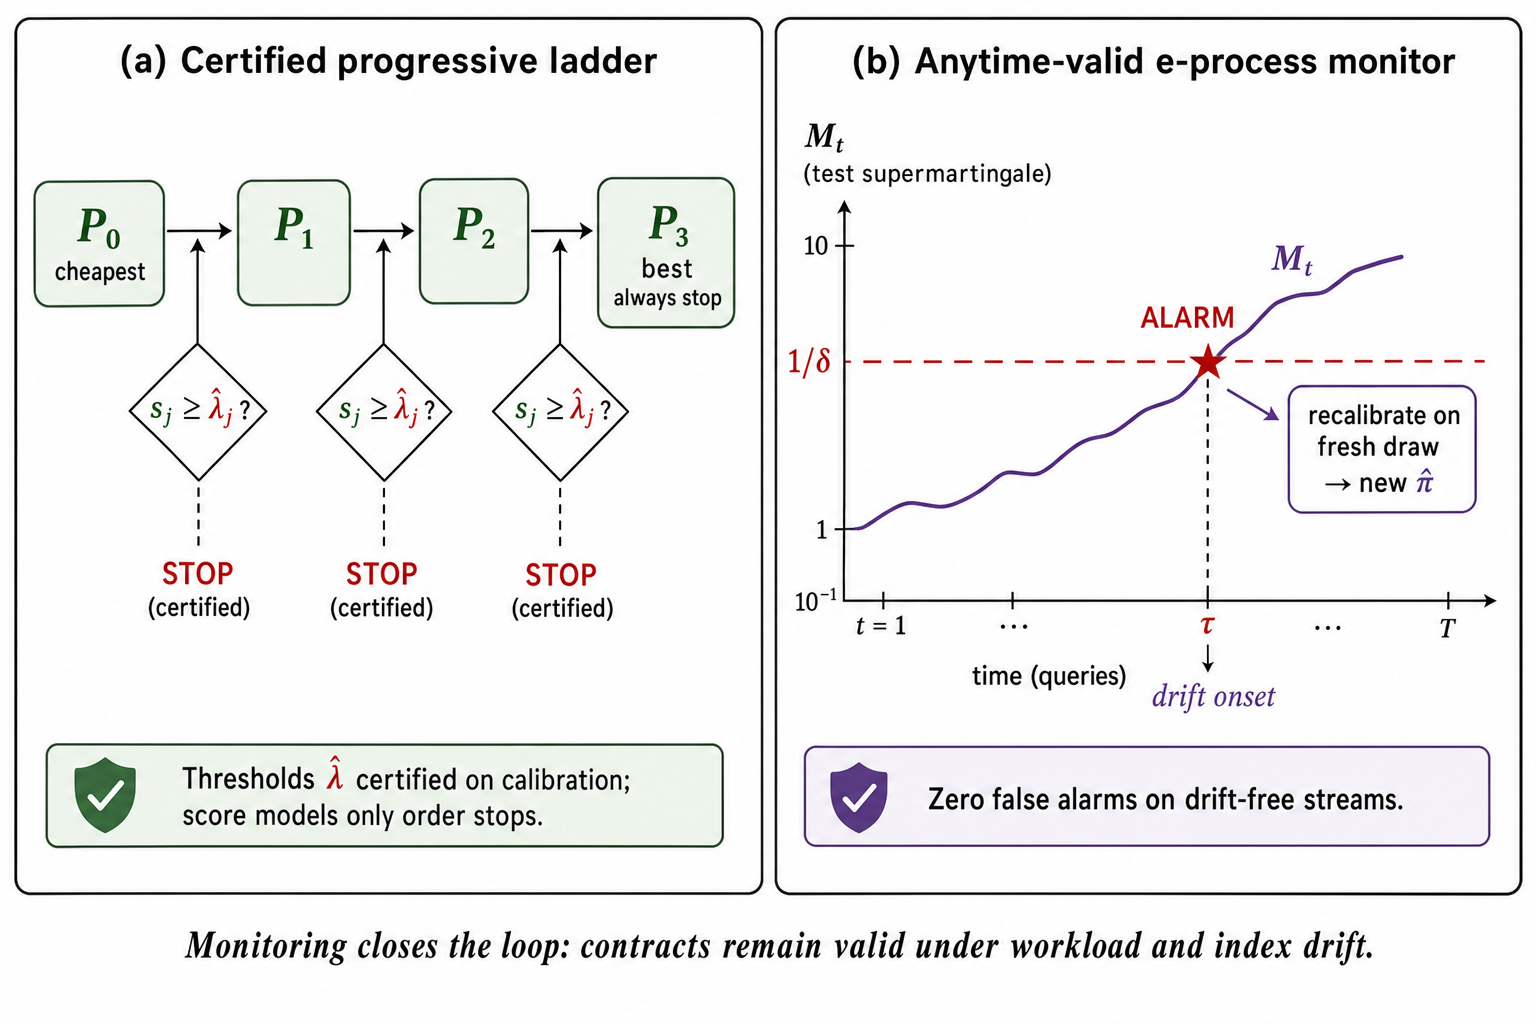
\includegraphics[width=0.95\textwidth]{figures/fig_runtime_imagegen.png}
\caption{Progressive execution and online monitoring.
(a)~A certified escalation ladder stops at the first rung whose
sufficiency score clears the calibration-certified threshold
$\hat\lambda_j$; scores only order stops, thresholds carry the
guarantee (Theorem~\ref{thm:validity}).
(b)~The anytime-valid e-process $M_t$ alarms when it crosses
$1/\delta$, triggering recalibration; under the contract it has
false-alarm probability $\le\delta$ (Proposition~\ref{prop:eprocess}).}
\Description{A progressive execution ladder escalates through stronger
plans, while an anytime-valid monitor observes audited contract losses
and triggers recalibration after a detected shift.}
\label{fig:runtime}
\end{figure*}


\subsection{Progressive and group-aware execution}

A progressive policy reuses evidence while moving up the ladder. A query
stops at rung $j$ when its runtime sufficiency score clears the certified
threshold; otherwise it executes the next, stronger plan. We charge the
cumulative cost of all visited rungs, even though retrieval, fusion, and
reranking state can be reused. The policy, including its stopping rule, is
the object certified by Theorem~\ref{thm:validity}.

Marginal control may hide failures on a known slice, such as CRAG queries
whose answers change in real time. For a grouping
$G(q)\in\{1,\ldots,m\}$, \system can learn a policy per group and certify it
on that group's calibration records at level $\delta/m$. A union bound then
gives simultaneous conditional guarantees
$R_j(\hat\pi\mid G=g)\leq\alpha_j$ for all groups. This option spends
statistical power to expose and price systematic differences.

\subsection{Anytime-valid monitoring}
\label{sec:monitor}

Calibration and deployment distributions may diverge because the query
mix changes, an index becomes stale, or an API degrades. \system monitors
audited losses $\ell_t\in[0,1]$ using a restart-mixture
e-process~\cite{ramdas2023savi,shin2024edetectors}. For horizon $T$, restart
time $r$, and bet $w\in W\subset(0,1/\alpha)$, define
\[
E_t^{(r,w)}=\prod_{i=r}^{t}(1+w(\ell_i-\alpha)).
\]
The detector mixes every possible restart instead of taking a
data-dependent maximum:
\begin{equation}
\label{eq:mixdetector}
M_t=\sum_{r=1}^{t}\sum_{w\in W}\frac{E_t^{(r,w)}}{T|W|}
      +\left(1-\frac{t}{T}\right).
\end{equation}
The last term is the prior mass of restarts not yet active. The recursion
$A_t^{(w)}=(A_{t-1}^{(w)}+1/(T|W|))
(w(\ell_t-\alpha))(A_{t-1}^{(w)}+1/(T|W|))$
updates the mixture in $O(|W|)$ time and space per audited query.

\begin{proposition}[Anytime validity]
\label{prop:eprocess}
If $\E[\ell_t\mid\mathcal F_{t-1}]\leq\alpha$ for all $t$, then
$\Prob(\exists t\leq T:M_t\geq1/\delta)\leq\delta$.
\end{proposition}
\begin{proof}
Each factor has conditional expectation at most one, hence every
$E_t^{(r,w)}$ is a nonnegative supermartingale. Equation~\ref{eq:mixdetector}
is a fixed convex mixture of these processes and has initial value one.
Ville's inequality gives the result.
\end{proof}

A restart born near a changepoint is not suppressed by the compliant
history before it. If the post-change mean is $\alpha'>\alpha$ and
$g^\star=\max_{w\in W}\E[\log(1+w(\ell_t-\alpha))]>0$, standard bounded
increment concentration gives detection delay
\[
O\!\left(
\frac{\log(1/\delta)+\log(T|W|)+\log(1/\delta')}{g^\star}
\right)
\]
with probability $1-\delta'$. The bound is independent of the change time.
A CUSUM-style companion recursion records the start of the current
positive-growth run to estimate the changepoint; it is used only for
diagnosis, not validity.

\subsection{Recertification loop}

On an alarm, \system enters a strongest-plan fallback, collects a labeled
post-alarm window, and reruns the fixed-sequence test. A new policy is
deployed only after it is certified on that window; if no candidate is
feasible, the system reports this result and continues with the fallback.
For repeated epochs, a geometric schedule
$\delta_k=\delta/2^{k+1}$ splits each epoch's budget between certification
and monitoring. Since $\sum_k\delta_k=\delta$, a union bound covers an
unbounded sequence of alarms and scheduled horizon restarts.

Monitoring need not audit every query. If each query is sampled
independently with probability $r$, the audited subsequence preserves the
conditional-mean null and therefore the guarantee. Detection delay grows
by approximately $1/r$ in wall-clock queries, making audit rate a direct
cost--reaction-time control.
